% A LaTeX (non-official) template for ISAE projects reports
% Copyright (C) 2014 Damien Roque
% Version: 0.2
% Author: Damien Roque <damien.roque_AT_isae.fr>

\documentclass[11pt,a4paper]{report}
\usepackage[utf8]{inputenc}
\usepackage[T1]{fontenc}
%\usepackage[frenchb]{babel} % If you write in French
\usepackage[english]{babel} % If you write in English
\usepackage{a4wide}
\usepackage{graphicx}
\graphicspath{{images/}}
%\usepackage{subfig}
\usepackage{tikz}
\usetikzlibrary{shapes,arrows}
\usepackage{pgfplots}
\pgfplotsset{compat=newest}
\pgfplotsset{plot coordinates/math parser=false}
\newlength\figureheight
\newlength\figurewidth
\pgfkeys{/pgf/number format/.cd,
set decimal separator={,\!},
1000 sep={\,},
}
\usepackage{ifthen}
\usepackage{ifpdf}
\ifpdf
\usepackage[pdftex]{hyperref}
\else
\usepackage{hyperref}
\fi
\usepackage{color}
\hypersetup{%
colorlinks=true,
linkcolor=black,
citecolor=black,
urlcolor=black}

\renewcommand{\baselinestretch}{1.05}
\usepackage{fancyhdr}
\pagestyle{fancy}
\fancyfoot{}
\fancyhead[LE,RO]{\bfseries\thepage}
\fancyhead[RE]{\bfseries\nouppercase{\leftmark}}
\fancyhead[LO]{\bfseries\nouppercase{\rightmark}}
\setlength{\headheight}{15pt}

\let\headruleORIG\headrule
\renewcommand{\headrule}{\color{black} \headruleORIG}
\renewcommand{\headrulewidth}{1.0pt}
\usepackage{colortbl}
\arrayrulecolor{black}

\fancypagestyle{plain}{
  \fancyhead{}
  \fancyfoot[C]{\thepage}
  \renewcommand{\headrulewidth}{0pt}
}

\makeatletter
\def\@textbottom{\vskip \z@ \@plus 1pt}
\let\@texttop\relax
\makeatother

\makeatletter
\def\cleardoublepage{\clearpage\if@twoside \ifodd\c@page\else%
  \hbox{}%
  \thispagestyle{empty}%
  \newpage%
  \if@twocolumn\hbox{}\newpage\fi\fi\fi}
\makeatother

\usepackage{textgreek}
\usepackage{amsthm}
\usepackage{amssymb,amsmath,bbm}
\usepackage{array}
\usepackage{bm}
\usepackage{multirow}
\usepackage[footnote]{acronym}
\usepackage{subcaption}
\usepackage{amsmath}
%\usepackage{mathtools}
\usepackage{multicol}
\usepackage{algorithm}
\usepackage{algorithmic}

\newcommand*{\SET}[1]  {\ensuremath{\mathbf{#1}}}
\newcommand*{\VEC}[1]  {\ensuremath{\boldsymbol{#1}}}
\newcommand*{\FAM}[1]  {\ensuremath{\boldsymbol{#1}}}
\newcommand*{\MAT}[1]  {\ensuremath{\boldsymbol{#1}}}
\newcommand*{\OP}[1]  {\ensuremath{\mathrm{#1}}}
\newcommand*{\NORM}[1]  {\ensuremath{\left\|#1\right\|}}
\newcommand*{\DPR}[2]  {\ensuremath{\left \langle #1,#2 \right \rangle}}
\newcommand*{\calbf}[1]  {\ensuremath{\boldsymbol{\mathcal{#1}}}}
\newcommand*{\shift}[1]  {\ensuremath{\boldsymbol{#1}}}

\newcommand{\eqdef}{\stackrel{\mathrm{def}}{=}}
\newcommand{\argmax}{\operatornamewithlimits{argmax}}
\newcommand{\argmin}{\operatornamewithlimits{argmin}}
\newcommand{\ud}{\, \mathrm{d}}
\newcommand{\vect}{\text{Vect}}
\newcommand{\sinc}{\ensuremath{\mathrm{sinc}}}
\newcommand{\esp}{\ensuremath{\mathbb{E}}}
\newcommand{\hilbert}{\ensuremath{\mathcal{H}}}
\newcommand{\fourier}{\ensuremath{\mathcal{F}}}
\newcommand{\sgn}{\text{sgn}}
\newcommand{\intTT}{\int_{-T}^{T}}
\newcommand{\intT}{\int_{-\frac{T}{2}}^{\frac{T}{2}}}
\newcommand{\intinf}{\int_{-\infty}^{+\infty}}
\newcommand{\Sh}{\ensuremath{\boldsymbol{S}}}
\newcommand{\C}{\SET{C}}
\newcommand{\R}{\SET{R}}
\newcommand{\Z}{\SET{Z}}
\newcommand{\N}{\SET{N}}
\newcommand{\K}{\SET{K}}
\newcommand{\reel}{\mathcal{R}}
\newcommand{\imag}{\mathcal{I}}
\newcommand{\cmnr}{c_{m,n}^\reel}
\newcommand{\cmni}{c_{m,n}^\imag}
\newcommand{\cnr}{c_{n}^\reel}
\newcommand{\cni}{c_{n}^\imag}
\newcommand{\tproto}{g}
\newcommand{\rproto}{\check{g}}
\newcommand{\LR}{\mathcal{L}_2(\SET{R})}
\newcommand{\LZ}{\ell_2(\SET{Z})}
\newcommand{\LZI}[1]{\ell_2(\SET{#1})}
\newcommand{\LZZ}{\ell_2(\SET{Z}^2)}
\newcommand{\diag}{\operatorname{diag}}
\newcommand{\noise}{z}
\newcommand{\Noise}{Z}
\newcommand{\filtnoise}{\zeta}
\newcommand{\tp}{g}
\newcommand{\rp}{\check{g}}
\newcommand{\TP}{G}
\newcommand{\RP}{\check{G}}
\newcommand{\dmin}{d_{\mathrm{min}}}
\newcommand{\Dmin}{D_{\mathrm{min}}}
\newcommand{\Image}{\ensuremath{\text{Im}}}
\newcommand{\Span}{\ensuremath{\text{Span}}}

\newtheoremstyle{break}
  {11pt}{11pt}%
  {\itshape}{}%
  {\bfseries}{}%
  {\newline}{}%
\theoremstyle{break}

%\theoremstyle{definition}
\newtheorem{definition}{Définition}[chapter]

%\theoremstyle{definition}
\newtheorem{theoreme}{Théorème}[chapter]

%\theoremstyle{remark}
\newtheorem{remarque}{Remarque}[chapter]

%\theoremstyle{plain}
\newtheorem{propriete}{Propriété}[chapter]
\newtheorem{exemple}{Exemple}[chapter]

\parskip=5pt
%\sloppy

\newcommand{\mychapter}[2]{
    \setcounter{chapter}{#1}
    \setcounter{section}{0}
    \chapter*{#2}
    \addcontentsline{toc}{chapter}{#2}
}

\begin{document}

%%%%%%%%%%%%%%%%%%
%%% First page %%%
%%%%%%%%%%%%%%%%%%

\begin{titlepage}
\begin{center}

\begin{figure}
	\centering
	\begin{minipage}{.33\textwidth}
		\centering
		
\includegraphics[width=0.6\textwidth]{logo_cnrs}\\[1cm]
	\end{minipage}%
	\begin{minipage}{.33\textwidth}
		\centering
		
\includegraphics[width=0.6\textwidth]{logo_ipnl}\\[1cm]
	\end{minipage}
	\begin{minipage}{.33\textwidth}
		\centering
		
\includegraphics[width=0.6\textwidth]{logo_ucbl}\\[1cm]
	\end{minipage}
\end{figure}

{\large Institut de Physique Nucléaire de Lyon\\ Internship carried out from 2018/03/12 to 2018/07/13 }\\[0.5cm]

{\large Master 2 internship report}\\[0.5cm]

% Title
\rule{\linewidth}{0.5mm} \\[0.4cm]
{ \huge \bfseries Signal and background discrimination in \textgamma+jet events, recorded by the CMS experiment at the LHC. \\[0.4cm] }
\rule{\linewidth}{0.5mm} \\[1.5cm]

% Author and supervisor
\noindent
\begin{minipage}{0.4\textwidth}
  \begin{flushleft} \large
    \emph{Author :}\\
    Maxime \textsc{Giraud}\\
%    M. Prénom \textsc{Nom}
  \end{flushleft}
\end{minipage}%
\begin{minipage}{0.4\textwidth}
  \begin{flushright} \large
    \emph{Supervisor :} \\
    Viola \textsc{Sordini}\\
%    Dr.~Prénom \textsc{Nom}
  \end{flushright}
\end{minipage}

\vfill

% Bottom of the page
{\large Version 0.1 du\\ \today}

\end{center}
\end{titlepage}

%%%%%%%%%%%%%%%%%%%%%%%%%%%%%
%%% Non-significant pages %%%
%%%%%%%%%%%%%%%%%%%%%%%%%%%%%
%
%
%\chapter*{Acknowledgments}
%Lorem ipsum dolor sit amet, consectetur adipiscing elit. Sed non risus. Suspendisse lectus tortor, dignissim sit amet, adipiscing nec, ultricies sed, dolor. Cras elementum ultrices diam. Maecenas ligula massa, varius a, semper congue, euismod non, mi. Proin porttitor, orci nec nonummy molestie, enim est eleifend mi, non fermentum diam nisl sit amet erat. Duis semper. Duis arcu massa, scelerisque vitae, consequat in, pretium a, enim. Pellentesque congue. Ut in risus volutpat libero pharetra tempor. Cras vestibulum bibendum augue. Praesent egestas leo in pede. Praesent blandit odio eu enim. Pellentesque sed dui ut augue blandit sodales. Vestibulum ante ipsum primis in faucibus orci luctus et ultrices posuere cubilia Curae; Aliquam nibh. Mauris ac mauris sed pede pellentesque fermentum. Maecenas adipiscing ante non diam sodales hendrerit. Ut velit mauris, egestas sed, gravida nec, ornare ut, mi. Aenean ut orci vel massa suscipit pulvinar. Nulla sollicitudin. Fusce varius, ligula non tempus aliquam, nunc turpis ullamcorper nibh, in tempus sapien eros vitae ligula. Pellentesque rhoncus nunc et augue. Integer id felis.
%
\clearpage
\tableofcontents

%\clearpage
%\listoffigures

\clearpage
\chapter*{Acronyms and abbreviations}
\begin{acronym}[CP-OFDMX] % Give the longest acronym here
\acro{IPNL}{Institut de Physique Nucléaire de Lyon}
\acro{CERN}{Centre Européen pour la Recherche Nucléaire}
\acro{LHC}{Large Hadron Collider}
\acro{CMS}{Compact Muon Solenoid}
\acro{MC}{Monte-Carlo}
\acro{MVA}{MultiVariate Analysis}
\acro{ANN}{Artificial Neural Network}
\end{acronym}

%%%%%%%%%%%%%%%%%%%%%%%%%%%%%%%%%%%%%%%%%%%%
%%% Content of the report and references %%%
%%%%%%%%%%%%%%%%%%%%%%%%%%%%%%%%%%%%%%%%%%%%

\pagestyle{fancy}

\cleardoublepage

\mychapter{0}{Introduction}
%\addcontentsline{toc}{section}{Introduction}
\markboth{Introduction}{Introduction}
%\label{chap:introduction}
%\minitoc

At the Compact Muon Solenoid are produced at high-energy, proton-proton collision. At these energy scale quarks and
gluons interact to form collimated jet of hadrons, called hadronics jets
This phenomenon allow us to probe the QCD and the proton structure but is very complexe to analyze.\\
One way to measure jets energy is to study \textgamma+jet events, on fig (\ref{gamma_jet}) the photon is prompt and balance the jet energy.

\begin{figure}[h!]
  \centering
  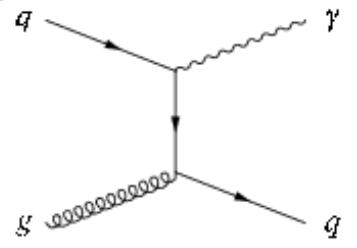
\includegraphics[width=0.4\textwidth]{gamma_jet}\\[1cm]
  \caption{Feynman diagram of a quark-gluon interaction, giving in output a high-energy quark and a prompt photon.}
  \label{gamma_jet}
\end{figure}

This report describes the analysis of \textgamma+jet events, in the first section will be described the CMS detector and
the hadronic jets. Then will be introduced the data that has been used for the analysis part.
For the analysis part will be implemented a multivariate analysis for photon identification this will be used for
measuring the \textgamma+jet purity in the data.

%%% Local Variables: 
%%% mode: latex
%%% TeX-master: "isae-report-template"
%%% End: 

\mychapter{1}{\textgamma+jet event classification in LHC collisions}
\label{chap:premierchapitre}

\section{CMS experiment at LHC}

The Compact Muon Solenoid (CMS) is a particle physics detector built on the Large Hadron Collider
(LHC) at CERN in switzerland and France. The goal of CMS experiment is to investigate the physics beyond the Standard
Model.
CMS is designed as a general-purpose detector, capable of studying many aspects of proton collisions at 0.9-13 TeV, the
center-of-mass energy of the LHC particle accelerator.\\
It is made of multiple particle detectors designed to measure the energy and momentum of products of the collisions.
The first layer called the "Tracker" reconstruct the paths of high-energy muons, electrons and hadrons as well as see
tracks coming from the decay of very short-lived particles.\\
Next the "Electromagnetic Calorimeter" is designed to measure with high accuracy the energies of electrons and
photons.\\
The Hadronic Calorimeter measures the energy of hadrons and provides indirect measurement of the presence of
non-interacting, uncharged particles such as neutrinos.\\
Theses layers all fit inside a large solenoid magnet of 3.8 Tesla, this allows the charge/mass ratio of particles to be
determined from the curved track that they follow in the magnetic field.
Finally the "Muon detectors and return yoke" are placed outside of the solenoid.

\section{Hadronic jets in proton-proton collisions}

In particle physics, jets are the experimental signatures of quarks and gluons produced in high-energy processes.\\
These particles having a net colour charge cannot exist freely due to couloour-confinement, thereby they are not
directly observed in nature. Instead, they come together to form colour-neutral hadrons by a process called
hadronisation that leads to a collimated spray of hadrons called a jet.
The detailed understanding of both the jet energy scale and of the transverse momentum resolution is of crucial
importance for many physics analyses.

%%% Local Variables: 
%%% mode: latex
%%% TeX-master: "isae-report-template"
%%% End: 

\mychapter{2}{Collision data}
\label{sec:unchapitre}

In this chapter will be described the data and simulations used for this study. Section 2.3 describes the input
variables that have been used for photon identification purpose.

\section{Monte-Carlo simulation}

We used simulated events for photon+jet and multijet production produced with the PYTHIA generator, interfaced to GEANT4 
for the simulation of the CMS detector. A special care is taken to accurately simulate the pileup contribution to well 
describe the data. The samples used in this study are official CMS samples.

\section{CMS data}

This study uses the full dataset collected by CMS in 2016 for proton-proton collisions. These data were data recorded with good 
LHC conditions and with a fully-functioning detector only, at $\sqrt{s} = 13 TeV$ for an integrated luminosity of $~ 36
fb^{-1}$.
 
\section{MVA variables}

We want to distinguish the so-called prompt photons, stemming for real photon+jet events, as the one from Fig.
(\ref{gamma_jet}, from photons produced inside jets during the hadronisation process and following decays. 
To this end, we dispose of several variables, representing various aspects of reconstructed photons\cite{CMS2015} :.

\begin{description}
    \item [Isolation variables] represent the total transverse momentum carried by additional objects (photons,charged hadron and neutral hadron) reconstructed
    in a fixed cone, around the processed photon, of radius $\Delta R$. These variables permit to discriminate between isolated
    prompt photons and neutral pions within a jet.
    \begin{description}
	    \item [Charged Hadron isolation (CHiso) : ] $I_{cha} = \sum_{cha_i}^{\Delta R}{p_{T,cha_i}}$ \\
            $cha_i$ corresponds to reconstructed charged hadron.
	    \item [Neutral Hadron isolation (NHiso) : ] $I_{neu} = \sum_{neu_i}^{\Delta R}{p_{T,neu_i}}$ \\
            $neu_i$ corresponds to reconstructed neutral hadron.
        \item [Photon isolation (Photoniso) : ] $I_\gamma = \sum_{\gamma_i}^{\Delta R}{p_{T,\gamma_i}}$ \\
            $\gamma_i$ corresponds to reconstructed photons, the sum doesn't account for the $p_T$ of the processed
            photon. (parler du pile-up avec $\rho$ ?)
	\\
    \end{description}
    \item [Shape variables] represent deposited energy shape in the ECAL.
    \begin{description}
    	\item [\textsigma\textsubscript{i\texteta i\texteta} :] Energy weighted spread within the 5x5 crystal matrix centred on the crystal with the largest energy deposit in the supercluster. Obtained by measuring position by countinig crystals. \\
		$ \sigma_{i \eta i \eta} = \sqrt{\frac{\sum^{5x5}_{j}\omega_j (i \eta_j - i \eta_{seed})^2}{\sum^{5x5}_{j}\omega_j}}$ \\
		$i \eta$ is the crystal index at position \texteta and $\omega_i$ is a weight representing the expected energy deposit measured.\\
		$i\eta_{seed} $ is the crystal with the largest energy deposit in the supercluster.\\
		$\omega_i = b + ln(\frac{E_i}{E_{5x5}})$
		\item [\textsigma\textsubscript{i\textphi i\textphi} :] same variable as $ \sigma_{i \eta i \eta}$ but computed in the \textphi direction.
		\item [\textsigma\textsubscript{i\texteta i\textphi} :] is the covariance between $ \sigma_{i \eta i \eta}$ and $ \sigma_{i \phi i \phi}$
    \\
		\item [\texteta\textsubscript{width} \: \textgamma :] Electromagnetic shower width in \texteta
    \item [\textphi\textsubscript{width} \: \textgamma :] Electromagnetic shower width in \textphi
	\item [R\textsubscript{9} \: \textgamma :] Energy sum of the 3x3 crystals centred on the most energetic crystal in
    the supercluster divided by the supercluster's energy. Lower values of R\textsubscript{9} for converted photons than those of unconverted photons.
	\item [Had/Em :] Hadronic calorimeter energy deposit over Electromagnetic calorimeter energy deposit
    \item [E\textsubscript{nxm}/E\textsubscript{5x5} :] Energy of most energetic nxm crystal set over energy of 5x5 crystal set
    \end{description}
    \item [\textrho :] Pile-up energy density, median of the transverse energy density per unit area.
\end{description}

%%% Local Variables: 
%%% mode: latex
%%% TeX-master: "isae-report-template"
%%% End: 

\mychapter{3}{Input variable analysis}
\label{sec:unchapitre}

A large set of variables is available from CMS data, they describe various aspect of photons and will be used to
distinguish between prompt and fragmentation photon.\\
To perform classification a multivariate analysis will be implemented, but MVA training can be time consuming and the "curse of
dimensionality" \footnote{Curse of dimensionality refers to problems that commonly arise when analyzing high-dimensionality data.
Increasing dimensionality lead to an increase of volume and so tends to scatter data points.} forces us to select the shortest possible input set.\\

Variables with most differences of shape for background and signal will be the most relevant for the MVA classification.
%\begin{description}
%    \item [Background vs Signal discrimination :] Variables with most differences of shape for background and signal will be picked.
%    \item [Low correlation between variables :] Needed in order to reduce redundancy of input data and thus will permit
%    to reduce MVA complexity (for example number of hidden neurons in ANN).
%\end{description}



The MVA will be trained with MC simulation for the signal sample and with the real data for the background sample. Indeed we trust MC simulation for the signal sample (\textgamma+jet events) but on the contrary MC backgound (multi-jet) may not be accurate (by not taking into account ...) and gave us low statistics.\\
For this reason real data will be used for the background sample and so a control region enriched in background event has to be defined (sideband).
In order to do that we need to perform a data-driven background estimation using a low-correlated variable for this sideband definition.

\section{Background vs Signal discrimination}

The choice of discriminating variables is done by looking at their shape for background and signal, processed from MC simulation.\\
Since the background is extracted from a data control region for the final analysis, a cross-check of the variables shape has to be done between Data and MC to validate this control region.\\
Fig. (\ref{NHiso_photon_dataVsMCbg}) shows an example of MC simulation and data comparison for \emph{neutral hadron isolation} variable. \\

\begin{figure}[h!]
  \centering
  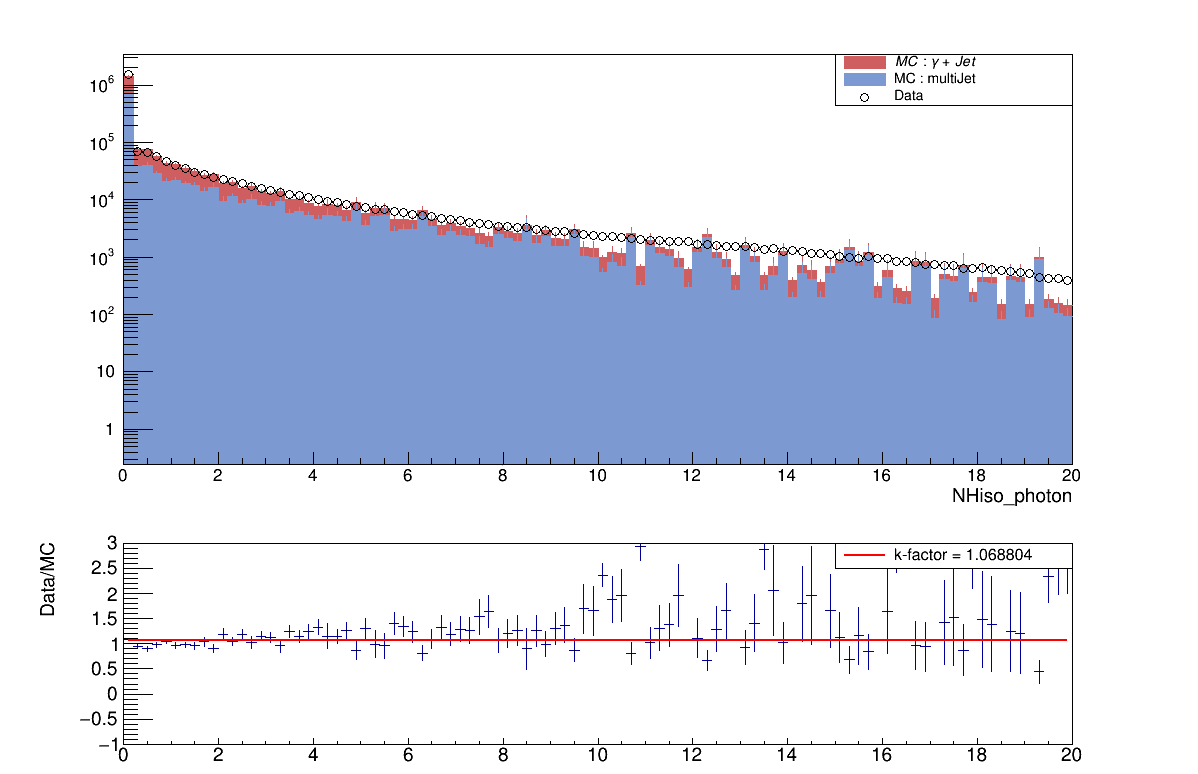
\includegraphics[width=0.8\textwidth]{NHiso_photon}\\[1cm]
  \caption{Top plot : Neutral hadron isolation variable for background (blue histogram) and signal MC (red histogram) and real data superimposed (empty circles). Normalized to integrated luminosity of $~36fb^{-1}$\\Bottom plot : Ratio of total expected events from MC (background+signal) over real data (blue cross) fitted by a constant (red line).}
  \label{NHiso_photon_dataVsMCbg}
\end{figure}

\section{Variable correlations}

%Training data needed-quantity increases with network complexity, so correlation between variables must be avoided in order to get the minimum redundancy.\\
Because we use distribution of the data in the control region as a proxy for their distribution in the signal region, we need to make sure that the variable for the sideband definition has low correlations with the other one. 
By looking at the correlation matrix fig. (\ref{corrMatrix_bgMC}) we can see that \emph{charged hadron isolation} is one good candidate and so will be used next for the sideband definition.\\

\begin{figure}[ht!]
  \centering
  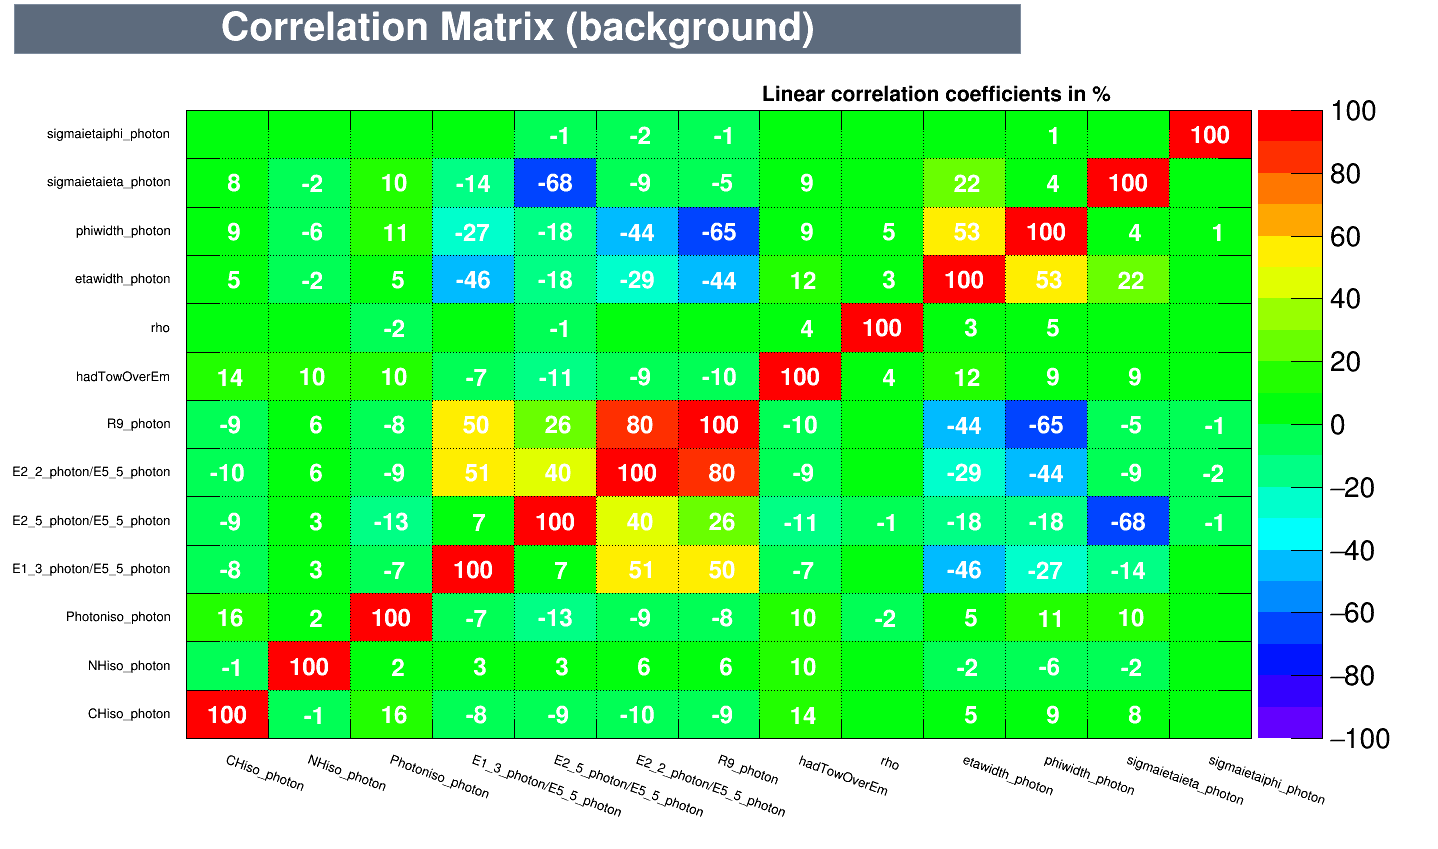
\includegraphics[width=0.7\textwidth]{corrMatrix_bgMC}\\[1cm]
  \caption{Correlation matrix for background MC, each line or column represent a variable.}
  \label{corrMatrix_bgMC}
\end{figure}

\section{Data driven background estimation}

An MVA will be performed with real data for the background, thereby a sideband (background enriched region in the data
sample) has to be defined on a low-correlated variable.\emph{Charged hadron isolation} fig. (\ref{sideband}) has been
chosen and the sideband defined in order to find a good compromise between background purity and number of events on data.
\begin{description}
	\item [Sideband definition]
	\begin{description}
    	\item 2.325 < \emph{Charge hadron isolation} < 15.
    	\item Background purity = 95.00 \%
		\item Number of events = $7.59*10^5$
	\end{description}
\end{description}

%Then a signal enriched region has been defined on the same variable, this cut will be applied on the signal data sample.
%\begin{description}
%	\item [Signal region definition]
%	\begin{description}
%    	\item \emph{Charge hadron isolation} < 2.
%    	\item Signal purity = ?? \%
%		\item Number of events = ??
%	\end{description}
%\end{description}

\begin{figure}[ht!]
  \centering
  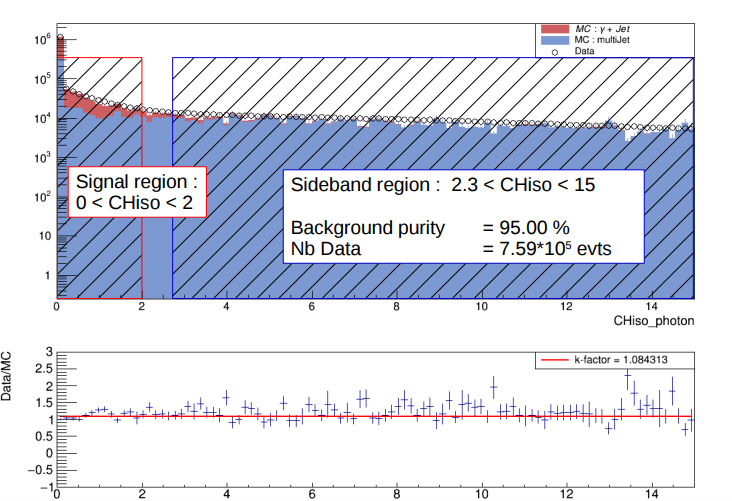
\includegraphics[width=0.7\textwidth]{sideband}\\[1cm]
  \caption{Charged hadron isolation for background MC (blue histogram), signal MC (red histogram) and real data
  superimposed (empty circles). Normalized to integrated luminosity of $~36fb^{-1}$\\On top of this is the sideband
  definition (red shaded area) and the signal region definition (blue shaded area)\\Bottom plot : Ratio of total expected events from MC (background+signal) over real data (blue cross) fitted by a constant (red line).}
  \label{sideband}
\end{figure}

For cross-check, we compare the variables shape for background MC in the signal region and DATA in the sideband region.
Fig. (\ref{MCbg_all_NHiso_photon}) shows an example of a comparison between \emph{neutral hadron isolation} for data in the sideband region and background Monte-Carlo. We can see a good agreement for MC and real data, except for a small trend in the high energy range probably due to the low statistics.
\begin{figure}[h!]
  \centering
  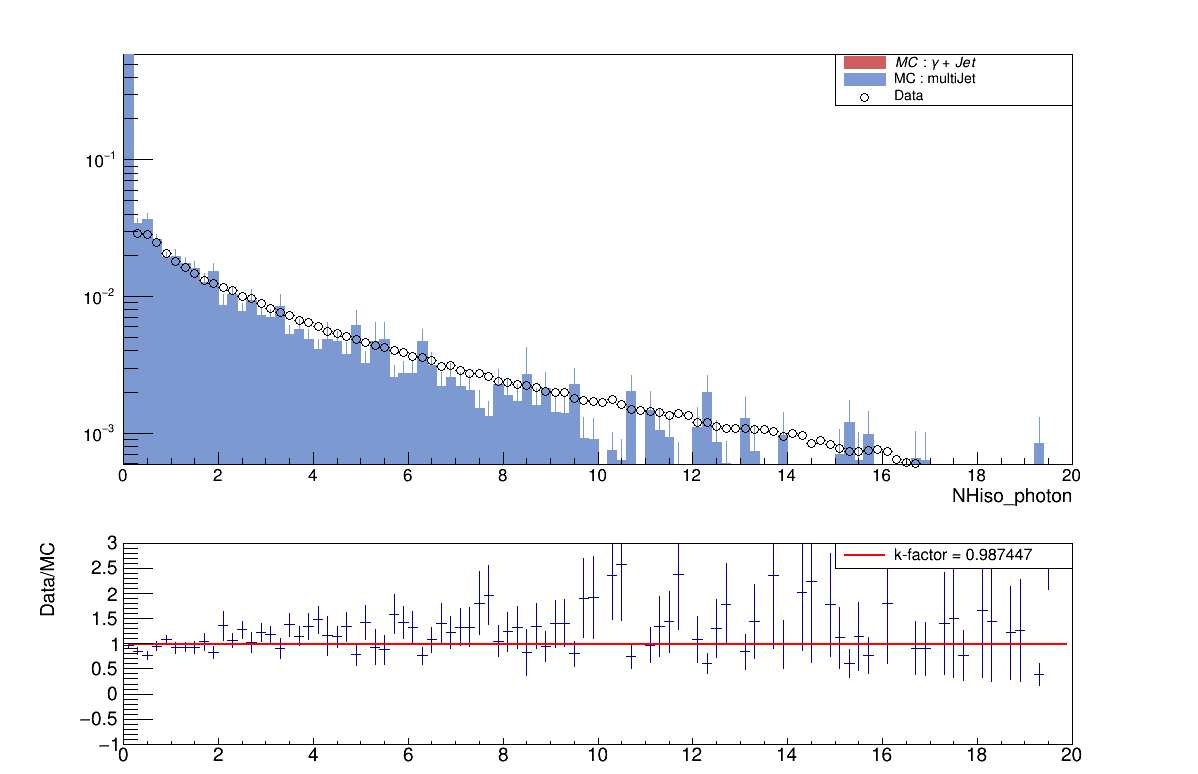
\includegraphics[width=0.7\textwidth]{MCbg_all_NHiso_photon}\\[1cm]
  \caption{Neutral hadron isolation for background MC (blue histogram) and real data in the sideband superimposed (empty circles). The integral of both distribution are normalized to unity.\\Bottom plot : Ratio of background MC over real data (blue cross) fitted by a constant (red line).}
  \label{MCbg_all_NHiso_photon}
\end{figure}

%%% Local Variables: 
%%% mode: latex
%%% TeX-master: "isae-report-template"
%%% End: 

\mychapter{4}{MultiVariate Analysis}
\label{sec:unchapitre}

Now that we get background and signal samples we can perform the MVA for classification.\\
For this purpose the TMVA framework from ROOT was used. Multiple MVA techniques were tested fig. (\ref{mva_multiple}) with default configuration then the 2
bests were selected for the tuning of their parameters : the ANN and BDT\\

\begin{figure}[h!]
\centering
    \begin{subfigure}[h!]{0.4\textwidth}
    \centering
        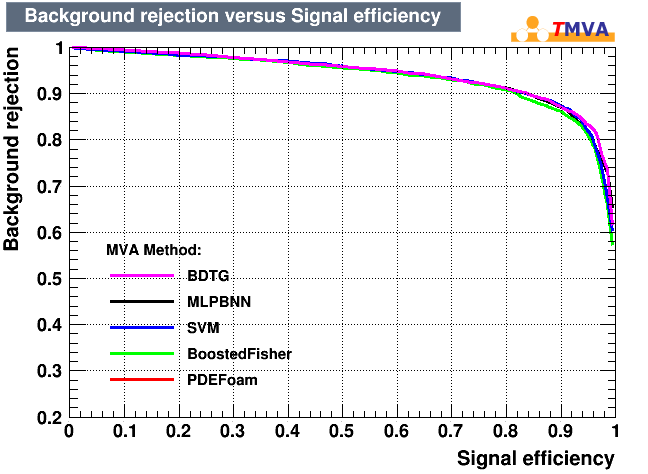
\includegraphics[width=\textwidth]{mva_multiple}
        \caption{ROC curves of 5 bests MVA, these are almost overlapping.}
        \label{mva_multiple}
  \end{subfigure}
  ~
    \begin{subfigure}[h!]{0.4\textwidth}
    \centering
        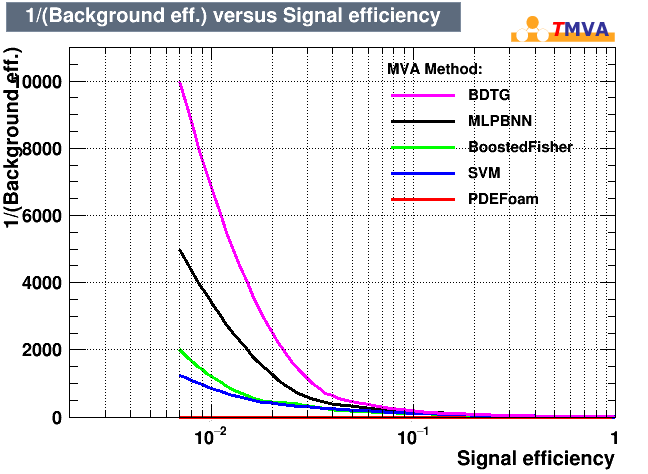
\includegraphics[width=\textwidth]{inv_mva_multiple.png}
        \caption{Inverse ROC curve for the 5 bests MVA, on this plot BDT and ANN(MLPBNN) are clearly the two bests.}
        \label{inv_mva_multiple}
  \end{subfigure}
  \caption{ROC curve for the 5 best MVA that has been tested. Receiver Operating Characteristic (ROC) curve reflects the discrimination power of a classifier. It is constructed by plotting the ratio of background rejection versus signal efficiency by varying a threshold on the MVA output.}
\end{figure}


\section{Artificial Neural Network}

An ANN is a multilayer perceptron with fully interconnected layers fig. (\ref{nn_arch}).
This ANN is used for classification, it is a function mapping an input vector $\vec{x_0}$ (input variables) to a scalar
$y$ with $y \in [0;1]$ (classification category).\\
Fig. (\ref{nn_output}) shows the output $y$ of the ANN that has been trained. Data have been divided in two, one
training sample and one testing sample.

%\subsection{Theory}

A neuron is referenced by his position in the network, a neuron $h_{i,j}(\vec{x_{j-1}}) \rightarrow h_{i,j}$ represent the i-th neuron of the j-th layer.\\
Such neuron sums all neuron's output in the (j-1)-th layer, weighted by their connection weight. This net sum is then evaluated through the activation function ( sigmoid, logistic, heaviside, linear, etc) fig. (\ref{one_neuron}).

\begin{figure}[h!]
\centering
    \begin{subfigure}[h!]{0.6\textwidth}
    \centering
    	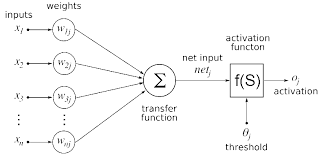
\includegraphics[width=\textwidth]{one_neuron}
    	\caption{Diagram of a single neuron algorithm.}
    	\label{one_neuron}
	\end{subfigure}
	~
    \begin{subfigure}[h!]{0.35\textwidth}
    \centering
    	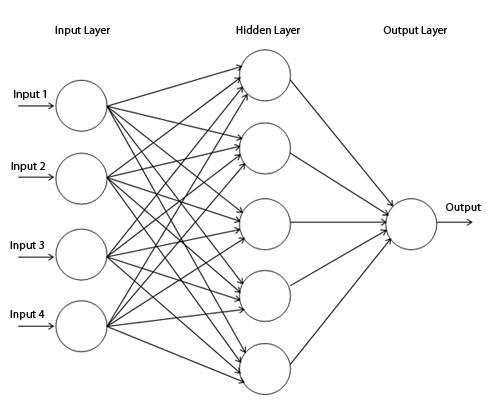
\includegraphics[width=\textwidth]{nn_arch}
    	\caption{Architecture of an artificial neural network with 4 input variables, one hidden layer, and one output neuron.}
    	\label{nn_arch}
	\end{subfigure}
\end{figure}


A lot of parameters are available for tuning :
\begin{description}
    \item [Input variables] Choice of input variable set, number of variables, choice of a Pre-processing method, etc.
    \item [ANN architecture] number of hidden layers, number of neurons per layer, choice of an activation function, etc.
    \item [Learning algorithm parameter] Choice of a learning method, choice of a regulator, value of learning rate, step size, weight decay rate, etc.
\end{description}

All of these cannot be optimize at the same time, so a choice has to be made.\\
The first parameter to be tune is the input variable set, a compromise has to be made in order to have the smallest input set but containing the most relevant information for classification.

\subsection{Input set optimization}

For this part an iterative process of optimization will be performed :
\begin{description}
	\item [step 1] Train MVA with full input variable set
	\item [step 2] Train N MVA removing one variable at a time
	\begin{description}
		\item [step 2.1] The MVA that succeed the best despite of having removed one variable, tells us that this variable wasn't revelant.
		\item [step 2.2] Remove this variable permanently, reiterate step 2 until no variable is left.
	\end{description}
	\item [final step] keep the input variable set of the best MVA
\end{description}

For evaluating the ANN multiple estimators has been tested :
\begin{description}
	\item [Mean Square Estimator (MSE)] $ MSE(\hat{\theta}) = E_{\hat{\theta}} [(\hat{\theta} - \theta)^2] =
    Var_{\hat{\theta}} + Bias(\hat{\theta}, \theta)^2$
	\item [Cross-Entropy (CE)] $ H(T,q) = -\sum_{i=1}^{N}{\frac{1}{N} log_2 q(x_i)}$
	\item [Overlapping criteria] is the sum of the products of signal and background response in each bin $ OC =
    \sum_{i=1}^{N}{signal_i*background_i} $ with $N :=$ number of bins , $signal_i := $ number of signal events in bin
    number i $background_i := $ number of background events in bin number i. Good classifiers show low value for this estimator.
\end{description}

\begin{figure}[h!]
\centering
    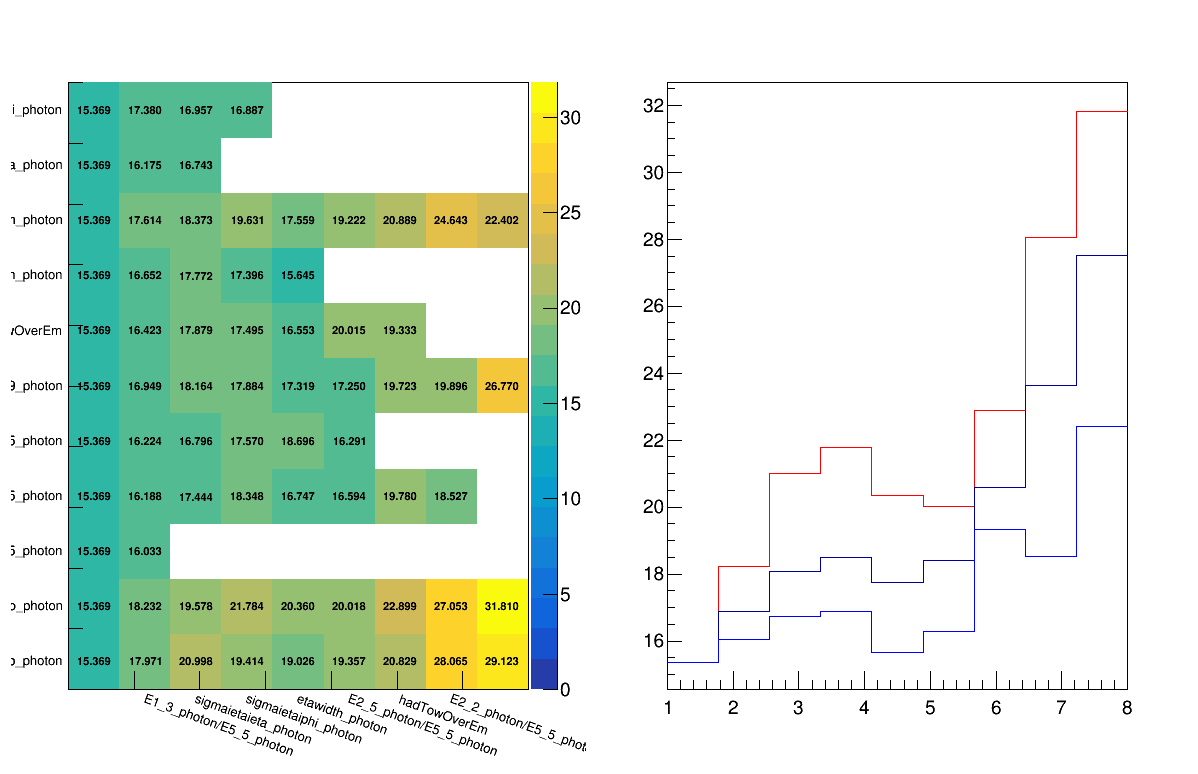
\includegraphics[width=1.\textwidth]{input_optim}
    \caption{On the left : Input variable set optimization results overview for the "overlapping criteria" estimator.
    Each bin is the estimator value for one MVA. Except for
    the 1st column that represents the MVA trained with the whole input seti (step 1), 2nd column
    represent MVA's that has been trained after removing one variable at a time (step 2), following columns are the
    iterations of step 2.\\
    On the right : overview of the estimator value for each column (step 2). maximum value (red solid line), average
    value (dark blue solid line) and lowest value (light blue solid line).}
    \label{input_optim}
\end{figure}

The optimization results in fig. (\ref{input_optim}) shows that keeping all the variables lead to the best MVA. So the whole input set will be used for the training. The ANN fig. (\ref{nn_output}) used 11 input variables : neutral hadron isolation, photon isolation, $\sigma_{i \eta i \eta}$, $\sigma_{i \eta i \phi}$, $\eta_{width}$, $\phi_{width}$, $R_9$, Had/Em, $E_{1x3}/E_{5x5}$, $E_{2x2}/E_{5x5}$ and $E_{2x5}/E_{5x5}$.
 
\begin{figure}[h!]
\centering
    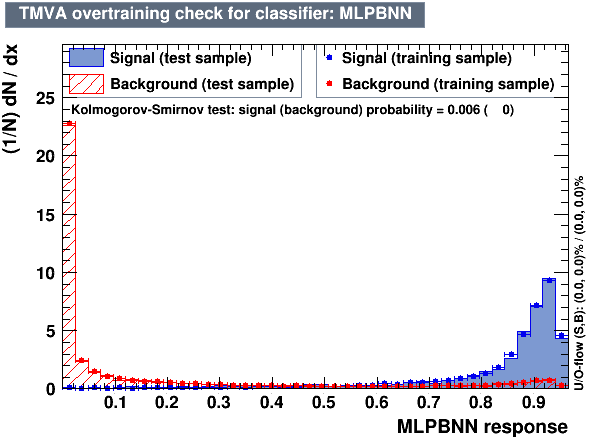
\includegraphics[width=0.6\textwidth]{nn_output}
    \caption{Artificial Neural Network response with signal from test sample (blue histogram), background from test
    sample (red shaded histogram), signal from training sample (blue dots) and background from training sample (red
    dots). The good agreement between training and testing sample shows no overfitting (in the case where these sample
    are representative of the data).}
    \label{nn_output}
\end{figure}

\section{Boosted Decision Tree}

Being the best MVA method a BDT has been trained also for the next part of the analysis fig. (\ref{bdt_output}).
BDT uses a decision tree in order to map from input variables to the event category (signal or background).
For this kind of classification tree, branches represent relations between variable or cuts on variables that lead to
leaf representing category of the event. Fig. (\ref{bdt_diagram}) shows an example diagram of a small BDT classifying
into 5 classes.\\
\begin{figure}[h!]
\centering
    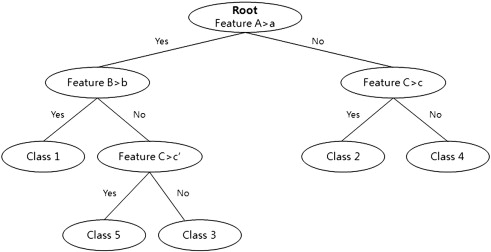
\includegraphics[width=0.6\textwidth]{bdt_diagram}
    \caption{Boosted Decision Tree classifying in 5 classes diagram.}
    \label{bdt_diagram}
\end{figure}


Multiple learning method has been used, the Gradient Boost Method was the most efficient one.
With this method, the classification is done by combining together weak classifiers in an iteratively way :
multiple "weak classifier" are trained and their output are combined in a weighted sum giving the "big classifier"
output, then at each iteration the "weak classifiers" weights are adjusted to minimize the error on classification.

\begin{figure}[h!]
\centering
    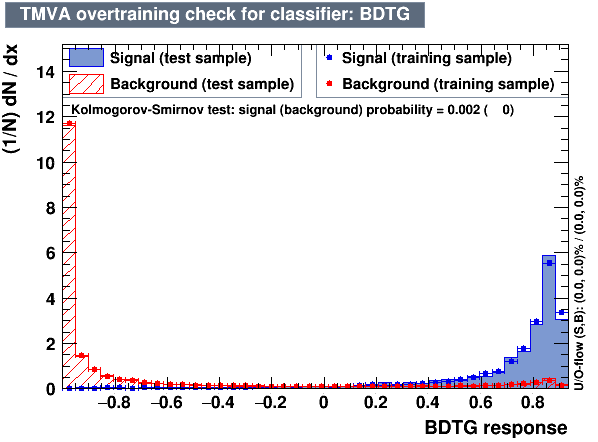
\includegraphics[width=0.6\textwidth]{bdt_output}
    \caption{Boosted Decision Tree response with signal from test sample (blue histogram),
    background from test sample (red shaded histogram), signal from training sample (blue dots)
    and background from training sample (red dots).}
    \label{bdt_output}
\end{figure}



%%% Local Variables: 
%%% mode: latex
%%% TeX-master: "isae-report-template"
%%% End: 


\mychapter{5}{Signal extracted on DATA}
\label{sec:unchapitre}

In this section will be extracted \textgamma+jet event purity on real data.
First we must establish PDF for signal (MC simulation) and background (real data in sideband), the analysis will be
performed on the $p_T^\gamma$ range [ ? ; ? ] divided in 11? bins

\section{Probability Density Function parametrization}

PDF are established using the ROOFit framework of ROOT using MC simulation for signal and real data in the sideband for the background.
Then ANN response for data in the signal region is expressed as : 

\begin{equation}
ANN(Data_{signal}) = a*PDF(MC_{signal}) + b*PDF(Data_{sideband})
\end{equation}

With : 
\begin{itemize}
	\item $ANN(Data_{signal}) :=$ the ANN response for Data in the signal region.
	\item $PDF(MC_{signal}) :=$ PDF for MC in the signal region.
	\item $PDF(Data_{sideband}) :=$ PDF for Data in the sideband. 
	\item $a :=$ number of signal events.
	\item $b :=$ number of background events. 
\end{itemize}

\begin{figure}[h!]
\centering
    
\includegraphics[width=0.5\textwidth]{coming_soon}
    \caption{Example of PDF parametrization for $p_T^\gamma \in [ ?;? ]$}
    \label{coming_soon}
\end{figure}

\section{Fit on Data}


\subsection{Pull-plot cross-check}

\subsection{\textgamma+jet events purity}


%%% Local Variables: 
%%% mode: latex
%%% TeX-master: "isae-report-template"
%%% End: 

\chapter*{Conclusion and future outlook}
\addcontentsline{toc}{chapter}{Conclusion and future outlook}
\markboth{Conclusion}{Conclusion}
\label{sec:conclusion}


%%% Local Variables: 
%%% mode: latex
%%% TeX-master: "isae-report-template"
%%% End: 



\appendix

\bibliographystyle{authoryear-fr}
\bibliography{references}

\clearpage


\begin{appendix}
	\chapter{MC vs data comparison}
	\chapter{Variable signal vs background discrimination}
    \chapter{Learning algorithms}
		\label{appendix:algo}
		\section{Back-Propagation}
		\section{Broyden-Fletcher-Goldfarb-Shanno (BFGS)}
		\section{Bayesian Regulator}
\end{appendix}

%%%%%%%%%%%%%%%%
%%% Abstract %%%
%%%%%%%%%%%%%%%%

\thispagestyle{empty}

\vspace*{\fill}
\noindent\rule[2pt]{\textwidth}{0.5pt}\\
{\textbf{Résumé ---}}
Lorem ipsum dolor sit amet, consectetur adipiscing elit. Sed non risus. Suspendisse lectus tortor, dignissim sit amet, adipiscing nec, ultricies sed, dolor. Cras elementum ultrices diam. Maecenas ligula massa, varius a, semper congue, euismod non, mi. Proin porttitor, orci nec nonummy molestie, enim est eleifend mi, non fermentum diam nisl sit amet erat. Duis semper. Duis arcu massa, scelerisque vitae, consequat in, pretium a, enim. Pellentesque congue. Ut in risus volutpat libero pharetra tempor. Cras vestibulum bibendum augue. Praesent egestas leo in pede. Praesent blandit odio eu enim. Pellentesque sed dui ut augue blandit sodales. Vestibulum ante ipsum primis in faucibus orci luctus et ultrices posuere cubilia Curae; Aliquam nibh. Mauris ac mauris sed pede pellentesque fermentum. Maecenas adipiscing ante non diam sodales hendrerit. Ut velit mauris, egestas sed, gravida nec, ornare ut, mi. Aenean ut orci vel massa suscipit pulvinar. Nulla sollicitudin. Fusce varius, ligula non tempus aliquam, nunc turpis ullamcorper nibh, in tempus sapien eros vitae ligula. Pellentesque rhoncus nunc et augue. Integer id felis.

{\textbf{Mots clés :}}
Lorem ipsum dolor sit amet, consectetur adipiscing elit. Sed non risus. Suspendisse lectus tortor.
\\
%\noindent\rule[2pt]{\textwidth}{0.5pt}
%\begin{center}
%  ISAE\\
%  10, avenue Édouard Belin\\
%  BP 54032\\
%  31055 Toulouse CEDEX 4
%\end{center}
%\vspace*{\fill}

\end{document}
